
\documentclass[12pt]{article}
\pagestyle{empty}
\setlength{\parskip}{0in}
\setlength{\textwidth}{6.8in}
\setlength{\topmargin}{-.5in}
\setlength{\textheight}{9.3in}
\setlength{\parindent}{0in}
\setlength{\oddsidemargin}{-.7cm}
\setlength{\evensidemargin}{-.7cm}

\usepackage{amsmath}
\usepackage{amsthm}
\usepackage{amstext}

\usepackage{graphicx}

\begin{document}


\textbf{MAT 105 Exam 1 (tan) Fall 2009} \hspace{.4in} {\large Name} \hrulefill

\begin{center}

\begin{tabular}
{|l|c|c|c|c|c|c|c|c|c|c|c|c|c|} \hline

 Problems & \hspace{5 pt} 1 \hspace{5 pt}  & \hspace{5 pt} 2 \hspace{5 pt} & \hspace{5 pt} 3 \hspace{5 pt} & \hspace{5 pt} 4 \hspace{5 pt} & \hspace{5 pt} 5 \hspace{5 pt} & \hspace{5 pt} Total  \hspace{5 pt} & &  \hspace{5 pt} Grade \hspace{5 pt}  \\ \hline
&&&&&&&&\\  
Points &&&&&&&    \hspace{.8in}\% &  \\ 
&&&&&&&& \\  \hline
Out of & 12 & 32 & 32 & 14 & 10 &100 & & \\ \hline

\end {tabular}

\end{center}

\vspace{.2in}

 \emph{Relax.  You have done problems like these before.  Even if these problems look a bit different, just do what you can.  If you're not sure of something, please ask! You may use your calculator.  Please show all of your work and write down as many steps as you can.  Don't spend too much time on any one problem.  Always remember to report the units on an answer. Do well.  And remember, ask me if you're not sure about something.}\\

\vspace{.5in} 
\noindent \emph{A few formulas from our book:}

\begin{center}

\textbf{Root Formula:} 

A solution of the equation $B^n=k$ is $B=k^{1/n}$.

\vspace{.2in} 

\textbf{Percent Increase Formula:} 

To get the result of increasing an amount by $r$\%, multiply by $1 + \frac{r}{100}$.

\end{center}

\hrulefill

%%%%%%%%%%%

\newpage
%%% Old 1.3, technology, fun
\begin{enumerate}
\item Video Casette Recorders (VCRs) used to be common in many households.  The graph below shows the percentage of households with a VCR ($H$, units of percentage) $Y$ years from 1978.  Use the graph to answer the following questions.

\begin{center}
\scalebox {.7} {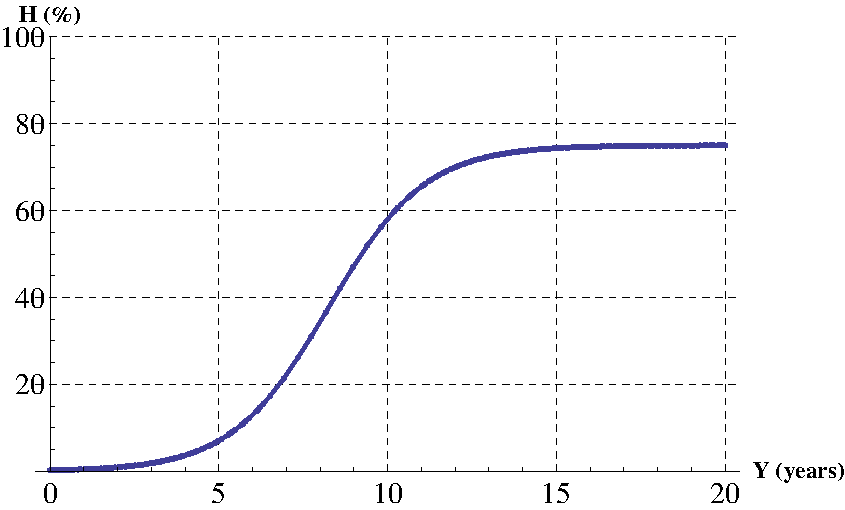
\includegraphics [width = 8in] {vcr}}
\end{center}



\begin{enumerate}
\item What percentage of households had a VCR in 1983 (5 years from 1978)?
\vfill
\item Does this graph show a dependency that is increasing, decreasing, or neither?
\vfill
\item Approximately in what year did the number of households with a VCR exceed 50\%?
\vfill
\item This graph only shows data to 1998.  If the graph continued to 2009, what do you think it would look like?  Describe your reasoning with a sentence or two.
\vfill
\end{enumerate}

%%%%%%%%%%%%%%%%%%%%%%%%%
\newpage
%%% Old 1.6, home, everyday
\item  I ordered some books online.  The cost for 3-day shipping was \$6.95.  For every book ordered, there was a fee of \$1.25.   

\begin{enumerate}
\item Make a table showing the shipping costs for 1 books, 2 books, and 10 books.
\vfill
\item Name the variables, including units, and write an equation illustrating the dependence.
\vfill
\item My total shipping charges were \$15.70.  Solve your equation to determine how many books I bought.  \emph{If you cannot solve the equation, you may show some other method of finding the answer for possible partial credit.}
\vfill
\item Draw a graph showing how the cost of my bill changes with the number of books ordered.
\vspace{.1in}
\begin{center}
\scalebox {.8} {
\includegraphics [width = 6in] {../GraphPaper}}
\end{center}
\vspace{.1in}
\end{enumerate}

%%%%%%%%%%%%%%%%%%%%%%%%%%%%%%%%%%%
\newpage

%%% Old 1.8, population, citizen?
\item The CIA world factbook estimated that the population of Costa Rica is growing at a rate of 1.3\% per year.  In 2008 the population was estimated to be 4.2 million.  

\begin{enumerate}
\item Write an equation illustrating this dependence using the following variables:

\quad $P= $ population (measured in millions of people)

\quad $Y = $ year (measured in years since 2008)

\vfill
\item Make a table showing the population in 2008, 2013, 2018, and 2023. Please report your answer to the first decimal place.
\vfill
\item Draw a graph showing how population will change in the future.
\vspace{.1in}
\begin{center}
\scalebox {.8} {
\includegraphics [width = 6in] {../GraphPaper}}
\end{center}
\vspace{.1in}
\item Use successive approximations to predict when the population will rise above 5 million.  Please report your answer to the first decimal place.   \emph{Display your work in a table.  Answer to the nearest year.  Be sure to say the actual year.}
\vfill
\vfill
\end{enumerate}


%%%%%%%%%%%%%%%%%
\newpage
%%% Old 1.7, physics (ice growth - not bicycle brakes!), fun
%%% Assume that the ice grows at 1/6" inches per day.  y = sqrt(2 k t ), y' = k/y.
\item Every winter, ice forms on the lake near my house.  After the temperature is consistently below freezing, the ice thickness continually grows.  Sometimes it is so thick that you can even drive cars on the lake!  For my lake, $T=0.17D^2$, where $T$ is number of days, and $D$ is the depth of the ice (in inches). 
\begin{enumerate}
\item Make a table showing the time it takes for the ice to grow to a depth 5, 10, 15, and 20 inches.  Please report your answer to the first decimal place.
\vfill
\item Approximately how deep will the ice (in inches) be after 30 days? Please report your answer to the first decimal place.

\emph{You may use whatever method you prefer to answer the question, but please give an answer accurate to one decimal place.}
\vfill

\end{enumerate}

\noindent \hrulefill
%%% Old 1.4, gas prices, fun
\item In Saudi Arabia, gasoline prices are recorded in riyals/liter.  (The riyal is the currency of Saudi Arabia).  The average price of gasoline in Saudi Arabia is 0.45 riyals/liter.  What would that price be in terms of US dollars per gallon?

\emph{Useful facts:  \$1.00 $\approx$ 3.75 riyals and 1 gallon $\approx$ 3.8 liters }
\vfill


\end{enumerate}



%%%%%%%%%%%%%%%%

\newpage




\end{document}
